\documentclass[../main/main.tex]{subfiles}

\newdate{date}{07}{10}{2020}


\begin{document}


\chapter{Misura resistenza del termometro}

\marginpar{ \textbf{Laboratory 1.} \\  \displaydate{date}. \\ Compiled:  \today.}
Dopo aver ricevuto lo \textbf{scatolone fabbricone} con tutto il materiale necessario per l'intera esperienza di laboratorio, la lezione di oggi riguarda principalmente fare pratica con le saldature e iniziare l'assemblaggio del ponte di Wheatstone che servirà per misurare la resistenza del termometro. Quest'ultimo circuito una volta assemblato dobrà essere saldato nel module NIM. Questo modulo verrà inserito in un posto in cui possono essere selezionate varie tensioni.


\section{Pratica con la saldatura}

Per prima cosa notiamo che ci sono due tipi di fili diversi: il cosidetto monofilo (che è rigido) e il multifilo che è più flessibile. Quello che cambia è che se io prendo la stelafili e levo la ricopertura, per il primo c'è un solo filo di rame, mentre per il multifilo c'è un intreccio di fili di rame.

Per fare una buona saldatura bisogna tenere conto delle tolleranze meccaniche del filo. Infatti se ho un filo molto piccolo, per saldarlo con la basetta devo inserire tanto stagno facendo però fare attenzione a non rompere il filo stesso. Inoltre, bisogna cercare di pulire bene i componenti prima della saldatura.
Un'altro accorgimento è che devo scaldare sui 150-200° (lo stagno fornito fonde attorno a quella temperatura), poi bisogna collegare l'elemento del componente con la basetta che ha una massa molto maggiore (quindi capacità termica molto maggiore) rispetto al componente, quindi anzichè mettere il saldatore a contatto con il filo, metterlo al contatto con la base per non rompere il filo.


Adesso vogliamo saldare l'estremità del filo con la basetta. Far passare il filo e saldare. Un'altro accorgimento è che independentemente dal fatto che sia mono o multi filo bisogna fare la \textbf{prestagnatura}, cioè ricoprire uniformemente il filo con lo stagno prima di fare la saldatura vera e propria. In questo modo si perde più tempo, ma la resa è migliore, infatti c'è una notevole differenza tra saldare il filo pre stagnato e non stagnato.
Per dissaldare si utilizza la pompetta dopo aver scaldato nuovamente lo stagno.

\section{Ponte di Wheatstone}

Adesso vogliamo montare sulla basetta mobile un circuito Wheatstone resistivo, che per la nostra esperienza sarà fondamentale. Infatti è necessario calibrare correttamente il circuito per trovare i valori ottimali delle resistenze.

Nella lezione di oggi abbiamo iniziato a costruire un prototipo di Ponte di Wheatstone per prendere dimistichezza con la sua calibrazione. Infatti i valori delle resistenze scelte, come ad esempio \( R \), sono stati selezionati molto intuitivamente. Sarà necessario calcolare i valori ottimali per l'esperimento.

Per prima cosa bisogna realizzare un circuito come in Fig. \ref{fig:1_1}.
Abbiamo utilizzato le seguenti resistenze:
\begin{equation*}
  R_1=R_2=57.9 \, \Omega, \quad R_x=28.8\, \Omega
\end{equation*}
Per scegliere il valore di \( R_x \), essendo che questo nel nostro circuito sarà rappresentato dal termometro, abbiamo consultato una tabella che descrive l'andamento del rapporto \( R_x/R_0 \) all'aumentare della temperatura per il nostro materiale. Si ha che il valore di \( R_0 = 100 \, \Omega  \), mentre il rapporto delle due quantità a 90 K (circa la temperatura alla quale lavoreremo) risulta essere:
\begin{equation*}
  \frac{R_x}{R_0} = 0.24298 \longrightarrow R_x = 24.298 \, \Omega
\end{equation*}
Quindi si è cercata nel cassetto una resistenza che avesse un valore simile a questo teorico.

Per quanto riguarda la resistenza \( R_v \) abbiamo utilizzato la resistenza presente nel modulo NIM e l'abbiamo regolata ad un valore approssimativamente uguale al valore \( R_x \) come atteso teoricamente.

\begin{figure}[h!]
\centering
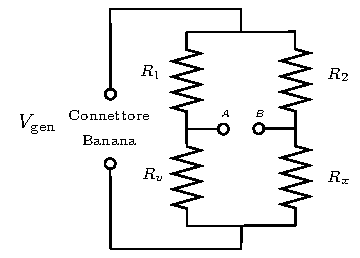
\includegraphics[width=0.5\textwidth]{../lessons/image/01/1.pdf}
\caption{\label{fig:1_1} Rappresentazione del ponte di Wheatstone.}
\end{figure}

\subsection{Calibrazione DC}
Per calibrare effettivamente il circuito bisogna effettuare prima una misura in \textbf{DC}. In questo caso la tensione \( V_{\text{gen}} \) è fornita dal generatore di tensione collegato attraverso i \textbf{cavi banana-banana}. Poi, per misurare la tensione ai vari capi delle resistenze si utilizza il tester digitale che ha una sensibilità del mV.

Affinchè il circuito sia calibrate in DC, dobbiamo variare il valore \( R_v \) fino a quando la tensione misurata ai capi \( B \) e \( A \) sia nulla, \( V_{BA} = 0\).
In particolare, la tensione \( V_{A} \) e \( V_{B} \) si può calcolare facilmente notando che sono dei partitori di tensione:
\begin{equation*}
  V_B = V_{\text{gen}} \frac{R_x}{R_2 + R_x}, \quad  V_A = V_{\text{gen}} \frac{R_v}{R_1+R_v}
\end{equation*}
Dall'analisi in DC abbiamo trovato che il valore che pone a zero la differenza di potenziale \( V_{AB}\) è \( R_v=28.8 \, \Omega  \).







\end{document}
